\section{Mathematical Model}
\label{sec:mathmod}

To model an infinitely long 3D waveguide \textit{in silico}, the simulation domain must be divided up into regions where specific mathematical relations hold. In this particular system there are three such regions (1) PEC surrounded dielectric, (2) Total Field / Scattered Field (TF/SF) 1-way source, and (3) Mur Absorbing Boundary Condition (Mur ABC). Regions (2)-(3) are essential as modeling an A high level diagram of a PEC bordered rectangular waveguide can be found in Fig. \ref{fig:model}(a) and a $\hat{y}$ sliced model where said relations hold can be found in Fig. \ref{fig:model}(b). These governing relations are then discretized to formulate time-stepping formulas which allow the system to evolve transiently.

\begin{figure}[t!]  
	\centering
	%the command within the [] sets the width of the figure, stability-condition is the jpg name
	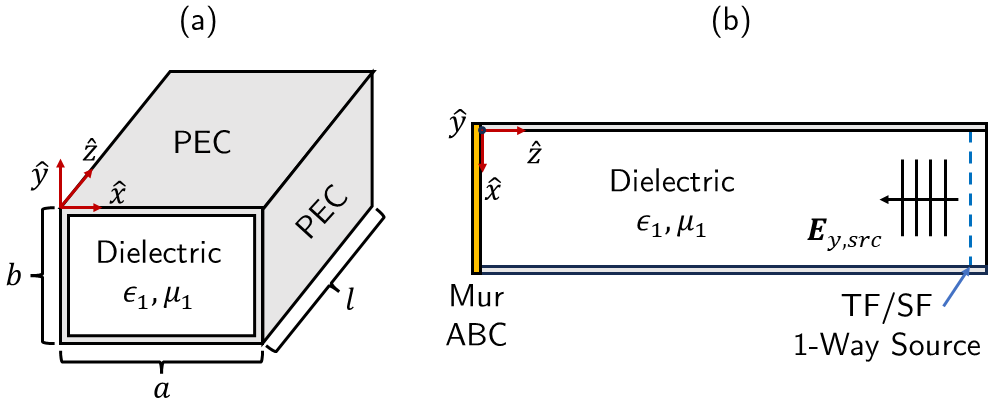
\includegraphics[width=0.9\linewidth]{model} 
	\caption{Diagrams of (a) High-Level PEC Rectangular Waveguide (b) $\hat{y}$-Sliced Model with Labeled Regions}
	\label{fig:model}
\end{figure}

\subsection{Model Formulation}
\label{subsec:model-formulation}

\subsubsection{PEC Surrounded Dielectric}
\label{subsec:dielectric-formulation}

As outlined in Fig. \ref{fig:model}(b) the vast majority of the simulation domain is composed of a PEC enclosed dielectric, the governing equations of which are Amp\`{e}re's and Faraday's Laws respectively. In differential form, these equations take the form 
\begin{align}
    \nabla\times\textbf{H} = \frac{\partial\textbf{D}}{\partial t} + \textbf{J}
    \label{eq:ampere}
\end{align}
and 
\begin{align}
    \nabla\times\textbf{E}=-\frac{\partial\textbf{B}}{\partial t} - \textbf{M}
    \label{eq:faraday}
\end{align}
where \textbf{E} is the electric field, \textbf{D} is the electric flux density, \textbf{H} is the electric field, \textbf{B} is the magnetic flux density, \textbf{J} is the free electric current density, and \textbf{M} is the fictitious free magnetic current density.

For simplicity, this analysis focuses on diagonally-isotropic, time-invariant, and non-dispersive dielectrics within the waveguide. Under these stipulations, each set of fields and flux densities, (\textbf{E}, \textbf{D}), (\textbf{H}, \textbf{B}), can be related using the following constitutive relations
\begin{align}
	\textbf{D}=\epsilon\textbf{E}, \textbf{B}=\mu\textbf{H}
	\label{eq:cor}
\end{align}
with $\epsilon$ and $\mu$ as the permittivity and permeability of the dielectric respectively.

In this analysis, no fictitious magnetic conductors will be considered as they are not pertinent, thus $\textbf{M} = 0$. The free electric current density is treated as a linear superposition of Ohmic conduction $\textbf{J}_{Ohm}=\sigma\textbf{E}$ and and a source term $\textbf{J}_{src}$
\begin{align}
	\textbf{J} = \sigma\textbf{E}
	\label{eq:ohm}
\end{align}
where $\sigma$ is the diagonally-isotropic, time-invariant dielectric conductivity. In the described system, the inclusion of both a source current density and ohmic current density is not necessary as the wave is assumed to already be propagating in the waveguide from the TF/SF source, and Ohmic losses result in evanescent wave propagation along the waveguide's length. Despite this, these current density terms will be included in the governing set of equations for completeness. The full set of governing equations for waves propogating within the dielectric are as follows
\begin{align}
    \nabla\times\textbf{H} = \epsilon\frac{\partial\textbf{E}}{\partial t} + \sigma\textbf{E} + \textbf{J}_{src}
    \label{eq:ampere-final}
\end{align}
\begin{align}
    \nabla\times\textbf{E}=-\mu\frac{\partial\textbf{H}}{\partial t}
    \label{eq:faraday-final}
\end{align}.

Each of these 3D vector equations can be broken down into $\hat{x}$, $\hat{y}$, and $\hat{z}$ component equations; the $\hat{y}$ components of \textbf{E} and \textbf{H} in Eqs. (\ref{eq:ampere-final})-(\ref{eq:faraday-final}) are
\begin{align}
	\frac{\partial H_x}{\partial z} - \frac{\partial H_z}{\partial x} = \epsilon\frac{\partial E_y}{\partial t} + \sigma E_y + J_{y,src}
	\label{ampere-full-ey}
\end{align}
and
\begin{align}
	\frac{\partial E_x}{\partial z} - \frac{\partial E_z}{\partial x} =-\mu\frac{\partial H_y}{\partial t}
	\label{faraday-full-hy}
\end{align}
respectively.

These scalar equations are valid for all locations within the dielectric region excluding those inside of the PEC at which there is a Dirichlet boundary condition
\begin{align}
	E_x=E_y=0.
	\label{eq:dirichlet}
\end{align}

\subsubsection{TF/SF 1-way Source}
\label{subsubsec:ftsf-mod}
To inject energy into this system, a TF/SF scheme is used. For this particular application, the $E_y$ field is used as a wave-port source (\textbf{TODO: EXPAND ME}). All total $E_y$ field values are considered as a superposition of source field $E_{y,src}$ and that of a scattered field $E_{y,scat}$ as
\begin{align}
	E_y = E_{y,src} + E_{y,scat}.
	\label{eq:tfsf-base}
\end{align}

https://www.tandfonline.com/doi/epdf/10.1163/156939300X00491?needAccess=true

ehere $E_{y,src}$ is injected into the system and the sca

Satisfying boundary conditoons